\documentclass{standalone}
\usepackage{tikz}
\usetikzlibrary{patterns, positioning}


\begin{document}
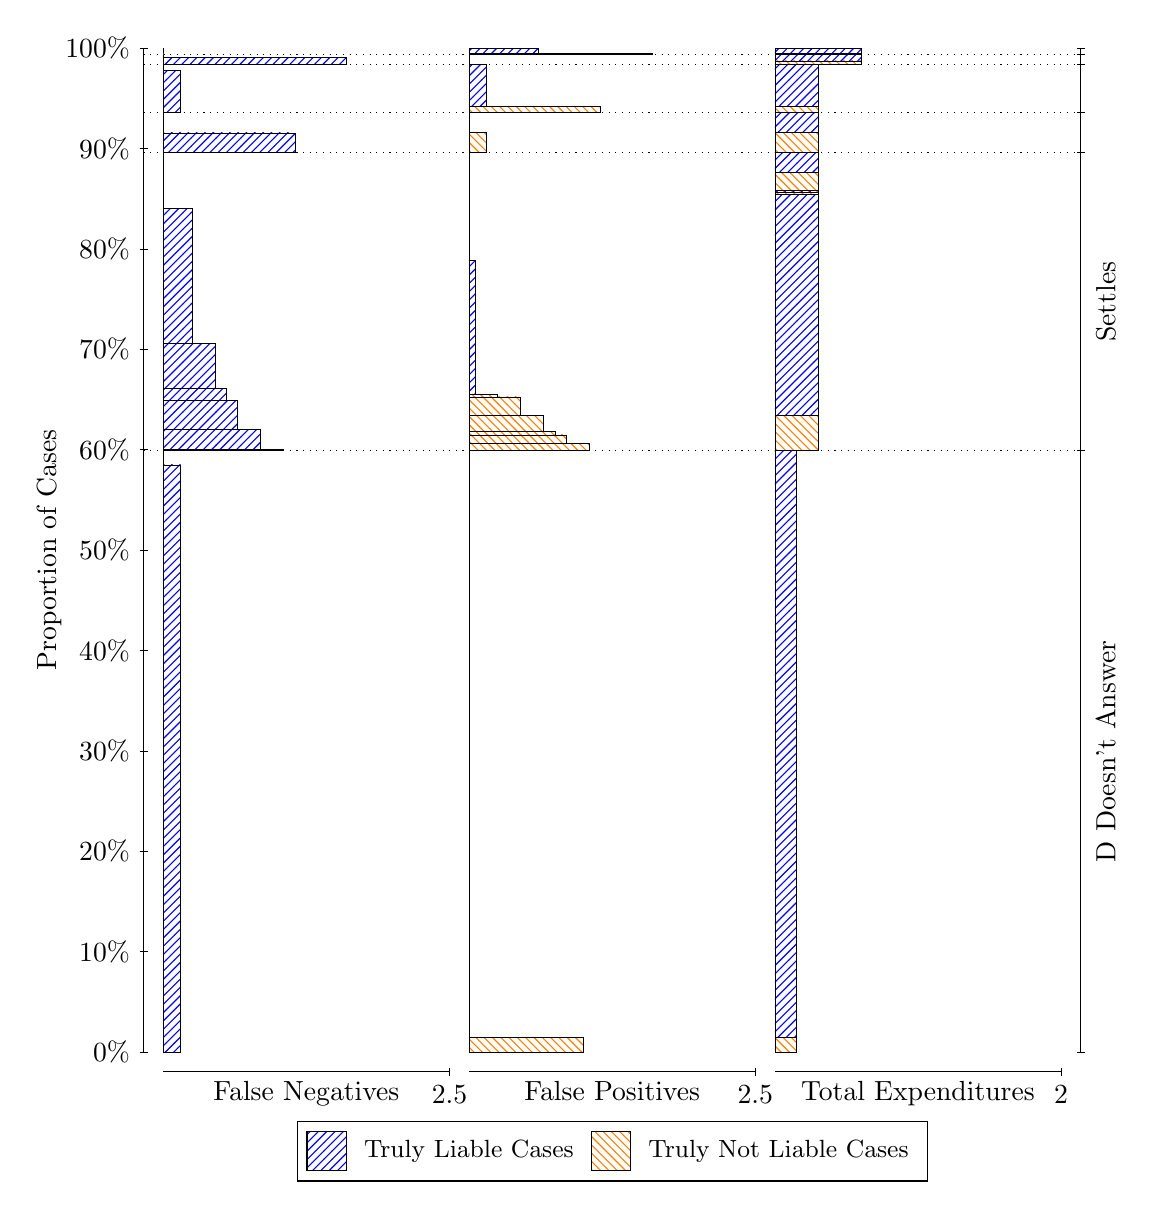
\begin{tikzpicture}
\draw[black, very thin] (1.5,1.75) -- (1.5,14.5);
\node[rotate=90, text=black, anchor=center] at (0.3, 8.125) {Proportion of Cases};
\draw[black, very thin] (1.45,1.75) -- (1.55,1.75);
\node[text=black, anchor=east] at (1.45, 1.75) {0\%};
\draw[black, very thin] (1.45,3.025) -- (1.55,3.025);
\node[text=black, anchor=east] at (1.45, 3.025) {10\%};
\draw[black, very thin] (1.45,4.3) -- (1.55,4.3);
\node[text=black, anchor=east] at (1.45, 4.3) {20\%};
\draw[black, very thin] (1.45,5.575) -- (1.55,5.575);
\node[text=black, anchor=east] at (1.45, 5.575) {30\%};
\draw[black, very thin] (1.45,6.85) -- (1.55,6.85);
\node[text=black, anchor=east] at (1.45, 6.85) {40\%};
\draw[black, very thin] (1.45,8.125) -- (1.55,8.125);
\node[text=black, anchor=east] at (1.45, 8.125) {50\%};
\draw[black, very thin] (1.45,9.4) -- (1.55,9.4);
\node[text=black, anchor=east] at (1.45, 9.4) {60\%};
\draw[black, very thin] (1.45,10.675) -- (1.55,10.675);
\node[text=black, anchor=east] at (1.45, 10.675) {70\%};
\draw[black, very thin] (1.45,11.95) -- (1.55,11.95);
\node[text=black, anchor=east] at (1.45, 11.95) {80\%};
\draw[black, very thin] (1.45,13.225) -- (1.55,13.225);
\node[text=black, anchor=east] at (1.45, 13.225) {90\%};
\draw[black, very thin] (1.45,14.5) -- (1.55,14.5);
\node[text=black, anchor=east] at (1.45, 14.5) {100\%};

\draw[black, very thin] (13.4,1.75) -- (13.4,14.5);
\draw[black, very thin] (13.35,1.75) -- (13.45,1.75);
\node[anchor=west] at (13.35, 1.75) {};
\draw[black, very thin] (13.35,9.3873) -- (13.45,9.3873);
\node[anchor=west] at (13.35, 9.3873) {};
\draw[black, very thin] (13.35,13.17) -- (13.45,13.17);
\node[anchor=west] at (13.35, 13.17) {};
\draw[black, very thin] (13.35,13.678) -- (13.45,13.678);
\node[anchor=west] at (13.35, 13.678) {};
\draw[black, very thin] (13.35,14.294) -- (13.45,14.294);
\node[anchor=west] at (13.35, 14.294) {};
\draw[black, very thin] (13.35,14.42) -- (13.45,14.42);
\node[anchor=west] at (13.35, 14.42) {};
\draw[black, very thin] (13.35,14.5) -- (13.45,14.5);
\node[anchor=west] at (13.35, 14.5) {};

\draw[black, very thin, pattern color=blue, pattern=north east lines] (1.75,1.75) rectangle (1.968,9.2065);
\draw[black, very thin, pattern color=orange, pattern=north west lines] (1.75,9.2065) rectangle (1.75,9.3873);
\draw[black, very thin, pattern color=blue, pattern=north east lines] (1.75,9.3873) rectangle (3.276,9.4047);
\draw[black, very thin, pattern color=blue, pattern=north east lines] (1.75,9.4047) rectangle (2.9853,9.6524);
\draw[black, very thin, pattern color=blue, pattern=north east lines] (1.75,9.6524) rectangle (2.6947,10.03);
\draw[black, very thin, pattern color=blue, pattern=north east lines] (1.75,10.03) rectangle (2.5493,10.178);
\draw[black, very thin, pattern color=blue, pattern=north east lines] (1.75,10.178) rectangle (2.404,10.747);
\draw[black, very thin, pattern color=blue, pattern=north east lines] (1.75,10.747) rectangle (2.1133,12.46);
\draw[black, very thin, pattern color=orange, pattern=north west lines] (1.75,12.46) rectangle (1.75,13.17);
\draw[black, very thin, pattern color=blue, pattern=north east lines] (1.75,13.17) rectangle (3.4213,13.423);
\draw[black, very thin, pattern color=orange, pattern=north west lines] (1.75,13.423) rectangle (1.75,13.678);
\draw[black, very thin, pattern color=blue, pattern=north east lines] (1.75,13.678) rectangle (1.968,14.215);
\draw[black, very thin, pattern color=orange, pattern=north west lines] (1.75,14.215) rectangle (1.75,14.294);
\draw[black, very thin, pattern color=blue, pattern=north east lines] (1.75,14.294) rectangle (4.0753,14.378);
\draw[black, very thin, pattern color=orange, pattern=north west lines] (1.75,14.378) rectangle (1.75,14.42);
\draw[black, very thin, pattern color=orange, pattern=north west lines] (1.75,14.42) rectangle (1.75,14.429);
\draw[black, very thin, pattern color=blue, pattern=north east lines] (1.75,14.429) rectangle (1.75,14.5);
\draw[black, very thin, pattern color=orange, pattern=north west lines] (5.6333,1.75) rectangle (7.0867,1.9308);
\draw[black, very thin, pattern color=blue, pattern=north east lines] (5.6333,1.9308) rectangle (5.6333,9.3873);
\draw[black, very thin, pattern color=orange, pattern=north west lines] (5.6333,9.3873) rectangle (7.1593,9.475);
\draw[black, very thin, pattern color=orange, pattern=north west lines] (5.6333,9.475) rectangle (6.8687,9.5862);
\draw[black, very thin, pattern color=orange, pattern=north west lines] (5.6333,9.5862) rectangle (6.7233,9.6331);
\draw[black, very thin, pattern color=orange, pattern=north west lines] (5.6333,9.6331) rectangle (6.578,9.8376);
\draw[black, very thin, pattern color=orange, pattern=north west lines] (5.6333,9.8376) rectangle (6.2873,10.07);
\draw[black, very thin, pattern color=orange, pattern=north west lines] (5.6333,10.07) rectangle (5.9967,10.097);
\draw[black, very thin, pattern color=blue, pattern=north east lines] (5.6333,10.097) rectangle (5.706,11.81);
\draw[black, very thin, pattern color=blue, pattern=north east lines] (5.6333,11.81) rectangle (5.6333,13.17);
\draw[black, very thin, pattern color=orange, pattern=north west lines] (5.6333,13.17) rectangle (5.8513,13.424);
\draw[black, very thin, pattern color=blue, pattern=north east lines] (5.6333,13.424) rectangle (5.6333,13.678);
\draw[black, very thin, pattern color=orange, pattern=north west lines] (5.6333,13.678) rectangle (7.3047,13.757);
\draw[black, very thin, pattern color=blue, pattern=north east lines] (5.6333,13.757) rectangle (5.8513,14.294);
\draw[black, very thin, pattern color=orange, pattern=north west lines] (5.6333,14.294) rectangle (5.6333,14.336);
\draw[black, very thin, pattern color=blue, pattern=north east lines] (5.6333,14.336) rectangle (5.6333,14.42);
\draw[black, very thin, pattern color=orange, pattern=north west lines] (5.6333,14.42) rectangle (7.9587,14.429);
\draw[black, very thin, pattern color=blue, pattern=north east lines] (5.6333,14.429) rectangle (6.5053,14.5);
\draw[black, very thin, pattern color=orange, pattern=north west lines] (9.5167,1.75) rectangle (9.7892,1.9308);
\draw[black, very thin, pattern color=blue, pattern=north east lines] (9.5167,1.9308) rectangle (9.7892,9.3873);
\draw[black, very thin, pattern color=orange, pattern=north west lines] (9.5167,9.3873) rectangle (10.062,9.8376);
\draw[black, very thin, pattern color=blue, pattern=north east lines] (9.5167,9.8376) rectangle (10.062,12.645);
\draw[black, very thin, pattern color=orange, pattern=north west lines] (9.5167,12.645) rectangle (10.062,12.672);
\draw[black, very thin, pattern color=blue, pattern=north east lines] (9.5167,12.672) rectangle (10.062,12.689);
\draw[black, very thin, pattern color=orange, pattern=north west lines] (9.5167,12.689) rectangle (10.062,12.922);
\draw[black, very thin, pattern color=blue, pattern=north east lines] (9.5167,12.922) rectangle (10.062,13.17);
\draw[black, very thin, pattern color=orange, pattern=north west lines] (9.5167,13.17) rectangle (10.062,13.424);
\draw[black, very thin, pattern color=blue, pattern=north east lines] (9.5167,13.424) rectangle (10.062,13.678);
\draw[black, very thin, pattern color=orange, pattern=north west lines] (9.5167,13.678) rectangle (10.062,13.757);
\draw[black, very thin, pattern color=blue, pattern=north east lines] (9.5167,13.757) rectangle (10.062,14.294);
\draw[black, very thin, pattern color=orange, pattern=north west lines] (9.5167,14.294) rectangle (10.607,14.336);
\draw[black, very thin, pattern color=blue, pattern=north east lines] (9.5167,14.336) rectangle (10.607,14.42);
\draw[black, very thin, pattern color=orange, pattern=north west lines] (9.5167,14.42) rectangle (10.607,14.429);
\draw[black, very thin, pattern color=blue, pattern=north east lines] (9.5167,14.429) rectangle (10.607,14.5);
\draw[black, dotted] (1.5,9.3873) -- (13.4,9.3873);
\draw[black, dotted] (1.5,13.17) -- (13.4,13.17);
\draw[black, dotted] (1.5,13.678) -- (13.4,13.678);
\draw[black, dotted] (1.5,14.294) -- (13.4,14.294);
\draw[black, dotted] (1.5,14.42) -- (13.4,14.42);
\draw[black, very thin] (1.75,1.5) -- (5.3833,1.5);
\node[text=black, anchor=north] at (3.5667, 1.5) {False Negatives};
\draw[black, very thin] (5.3833,1.45) -- (5.3833,1.55);
\node[text=black, anchor=north] at (5.3833, 1.45) {2.5};

\draw[black, very thin] (5.6333,1.5) -- (9.2667,1.5);
\node[text=black, anchor=north] at (7.45, 1.5) {False Positives};
\draw[black, very thin] (9.2667,1.45) -- (9.2667,1.55);
\node[text=black, anchor=north] at (9.2667, 1.45) {2.5};

\draw[black, very thin] (9.5167,1.5) -- (13.15,1.5);
\node[text=black, anchor=north] at (11.333, 1.5) {Total Expenditures};
\draw[black, very thin] (13.15,1.45) -- (13.15,1.55);
\node[text=black, anchor=north] at (13.15, 1.45) {2};

\node[text=black, centered, rotate=90] at (13.72, 5.5686) {D Doesn't Answer};
\node[text=black, centered, rotate=90] at (13.72, 11.278) {Settles};





\draw (7.449999999999999,1.5) node[draw=none] (baseCoordinate) {};
\begin{scope}[align=center]
        \matrix[scale=0.5, draw=black, below=0.5cm of baseCoordinate, nodes={draw}, column sep=0.1cm]{
            \node[rectangle, draw, minimum width=0.5cm, minimum height=0.5cm, pattern color=blue, pattern=north east lines] {}; &
            \node[draw=none, font=\small, text=black] (B) {Truly Liable Cases}; &
            \node[rectangle, draw, minimum width=0.5cm, minimum height=0.5cm, pattern color=orange, pattern=north west lines] {}; &
            \node[draw=none, font=\small, text=black] (B) {Truly Not Liable Cases}; \\
            };
\end{scope}

\end{tikzpicture}
\end{document}